\chapter{Исследовательская часть}

\section{Технические характеристики}

Технические характеристики устройства, на котором выполнялись замеры по времени:

\begin{itemize}
	\item Процессор: AMD Ryzen 5 4600H 3 ГГц \cite{amd}.
	\item Оперативная память: 16 ГБайт.
	\item Операционная система: Windows 10 Pro 64-разрядная система версии 22H2 \cite{windows}.
\end{itemize}

При замерах времени ноутбук был включен в сеть электропитания и был нагружен только системными приложениями.


\section{Демонстрация работы программы}

%Тут абзац со ссылкой на рисунок и описанием того, что на нём представлено/происходит
На рисунке \ref{img:demonstration} представлена демонстрация работы разработанного программного обеспечения, а именно показаны результаты вычислений расстояний Левенштейна и Дамерау-Левенштейна для строк <<скат>>, <<кот>> и <<красивый>>, <<карсивый>> соответственно.  
\clearpage
\begin{figure}[h]
	\centering
	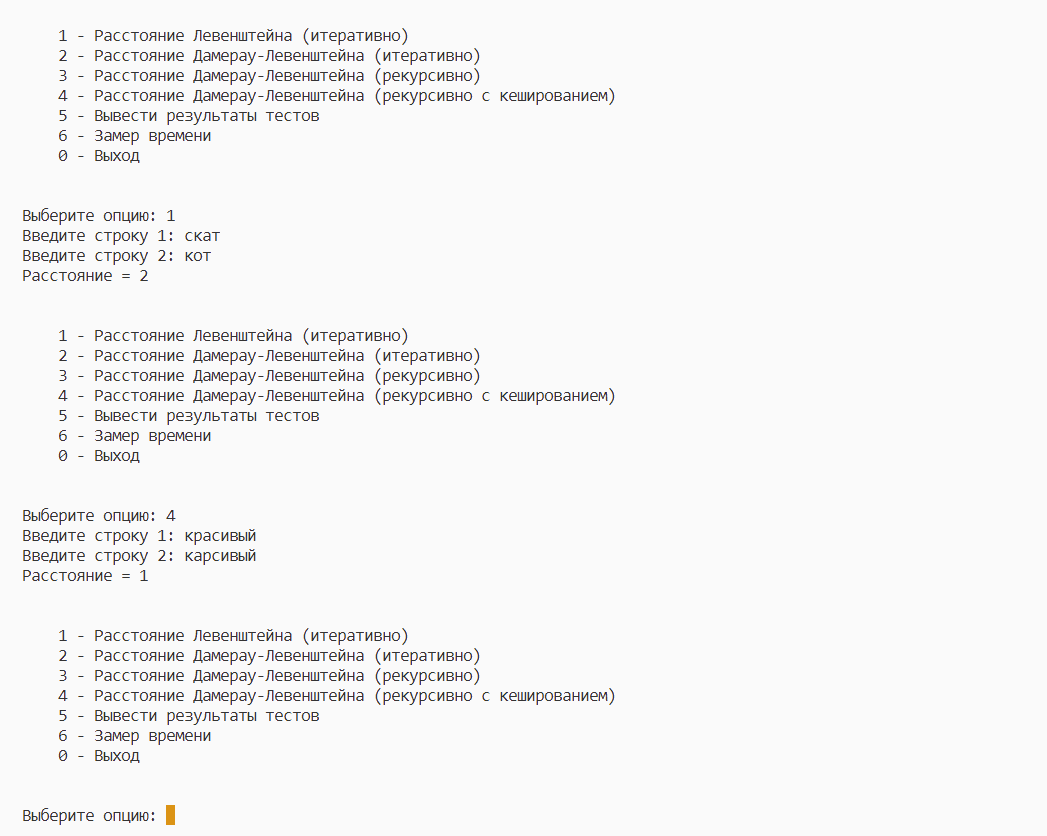
\includegraphics[height=0.7\textheight]{img/program.png}
	\caption{Демонстрация работы программы при поиске расстояний Левенштейна и Дамерау-Левенштейна}
	\label{img:demonstration}
\end{figure}

\clearpage

\section{Время выполнения алгоритмов}

Результаты замеров времени работы алгоритмов нахождения расстояний
Левенштейна и Дамерау–Левенштейна приведены в таблице \ref{tbl:time_measurements}. Замеры времени проводились на строках одинаковой длины и усреднялись для каждого набора одинаковых экспериментов.

\begin{table}[h]
	\begin{center}
		\begin{threeparttable}
			\captionsetup{justification=raggedright,singlelinecheck=off}
			\caption{Время работы алгоритмов (в секундах)}
			\label{tbl:time_measurements}
			\begin{tabular}{|c|c|c|c|c|}
				\hline
				Длина строк &  Л (и)  & Д-Л (и) & Д-Л (р) & Д-Л (рк) \\
				\hline
				1    & 0 & 0 & 0 & 0 \\ 
				\hline
				2    & 0	 & 1.56e-05 & 1.56e-05 & 0 \\ 
				\hline
				3    & 0.85e-06 & 1.56e-05 & 3.13e-05 & 1.56e-05 \\ 
				\hline
				4    & 1.56e-05 & 1.56e-05 &  1.72e-04 & 3.13e-05 \\ 
				\hline
				5    & 1.56e-05 & 1.56e-05 &  9.69e-04 & 4.69e-05 \\ 
				\hline
				6    & 1.56e-05 & 3.13e-05 & 5.11e-03 & 6.25e-05 \\ 
				\hline
				7    & 3.13e-05 & 3.13e-05 & 2.76e-02 & 9.38e-05 \\ 
				\hline
				8    & 4.69e-05  & 4.69e-05 & 1.52e-01  & 1.09e-04 \\ 
				\hline
				9    & 4.69e-05  & 6.25e-05 & 8.33e-01 & 1.25e-04 \\
				\hline
			\end{tabular}
		\end{threeparttable}
	\end{center}
\end{table}

\begin{figure}[h]
	\centering
	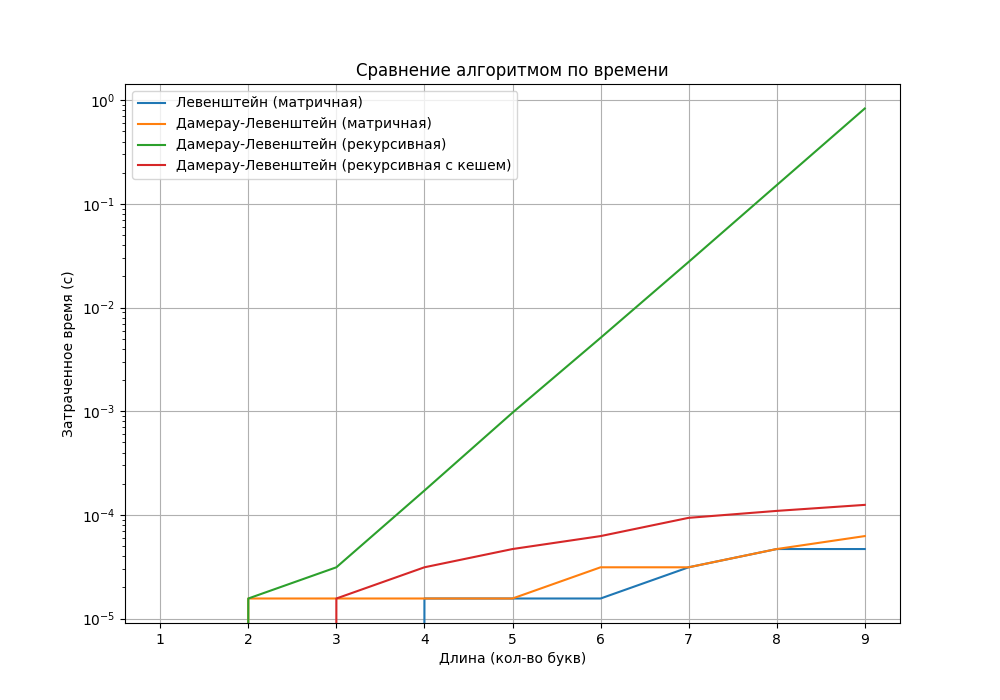
\includegraphics[width=0.7\textheight]{img/Figure_1.png}
	\caption{Сравнение алгоритмов по времени}
	\label{img:time}
\end{figure}

\clearpage

Наиболее эффективными являются алгоритмы, использующие матрицы, после них по скорости работы идет алгоритм использующий кеш, это обусловлено тем, что по сравнению с обычной рекурсией, мы не вычисляем повторно одни и те же значения, но все равно тратим время на рекурсивные вызовы. 

\section{Характеристики по памяти}

\label{memory}

Введем следующие обозначения:
\begin{itemize}
	\item $n$ -- длина строки $S_1$;
	\item $m$ -- длина строки $S_2$;
	\item $size()$ -- функция, вычисляющая размер в байтах;
	\item $int$ -- целочисленный тип данных;
	\item $string$ -- строковый тип данных.
\end{itemize}

Т.~к. алгоритмы, вычисляющие расстояния Левенштейна и Дамерау-Левенштейна, не отличаются по использованию памяти, то достаточно рассмотреть итеративную реализацию одного из этих алгоритмов, рекурсивную и рекурсивную с кешированием реализации алгоритмов вычисления расстояния Дамерау-Левенштейна.


Использование памяти при итеративной реализации теоритически равно:
\begin{equation}
	(n + 1) * (m + 1) * size(int) + 2 * size(string) + 2 * size(int),
\end{equation}
где 
\begin{itemize}
	\item $ (n + 1) * (m + 1) * size(int) $ -- хранение матрицы;
	\item $ 2 * size(string) $ -- хранение двух строк;
	\item $ 2 * size(int) $ -- адрес возврата и возвращаемое значение.
\end{itemize}


Максимальная глубина стека вызовов при рекурсивной реализации
нахождения расстояния Дамерау-Левенштейна равна сумме входящих строк,
соответственно, максимальный расход памяти равен:

\begin{equation}
	(n + m) * (2 * size(string) + 3 * size(int)),
\end{equation}
где 
\begin{itemize}
	\item $ (n + m) $ -- максимальная глубина стека вызовов;
	\item $ 2 * size(string) $ -- хранение двух строк;
	\item $ 2 * size(int) $ -- адрес возврата и возвращаемое значение;
	\item $ size(int) $ -- временная переменная.
\end{itemize}

Для алгоритма, использующего кеширование требуется дополнительно память под кеш и 4 временных переменных:

\begin{equation}
	(n + m) * (2 * size(string) + 6 * size(int)) + (n + 1) * (m + 1) * size(int),
\end{equation}
где 
\begin{itemize}
	\item $ (n + m) $ -- максимальная глубина стека вызовов;
	\item $ 2 * size(string) $ -- хранение двух строк;
	\item $ 2 * size(int) $ -- адрес возврата и возвращаемое значение;
	\item $ 4 * size(int) $ -- временные переменные;
	\item $ (n + 1) * (m + 1) * size(int) $ -- хранение кеша.
\end{itemize}

По расходу памяти итеративные алгоритмы проигрывают рекурсивным: максимальный размер используемой памяти в итеративном растет
как произведение длин строк, в то время как у рекурсивного алгоритма --
как сумма длин строк.


\section*{Вывод}

В данном разделе было произведено сравнение количества затраченного времени и памяти алгоритмов поиска расстояний Левенштейна и
Дамерау-Левенштейна. Наименее затратным по времени оказался итеративный алгоритм нахождения расстояния Левенштейна.

По таблице \ref{tbl:time_measurements} видно, что рекурсивный алгоритм в n раз проигрывает итеративному при длине строк 10. Поэтому рекурсивные алгоритмы следует использовать лишь при малых длинах строк.

При этом как было замечено в пункте \ref{memory}, рекурсивные алгоритмы занимают меньше памяти, чем итеративные алгоритмы.

Рекурсивная реализация алгоритма поиска расстояния Дамерау-Левенштейн будет более затратным по времени по сравнению с итеративной реализацией алгоритма поиска расстояния Дамерау-Левенштейна, но менее затратным по памяти по отношению к итеративному алгоритму Дамерау-Левенштейна. При этом рекурсивные алгоритм с кешированием проигрывает по памяти и по времени итеративному.